\chapter{Transformée de Laplace}	
\label{chap:laplace}	
	Dans le chapitre précédent, nous avons identifié deux manières de calculer la réponse transitoire d'un système :
	\begin{itemize}
		\item soit en considérant la réponse impulsionnelle et en calculant le produit de convolution dans le domaine temporel
		\item soit en considérant la fonction de transfert et en réalisant une simple multiplication dans le domaine fréquentiel, nécessitant une excitation exponentielle complexe.\\
	\end{itemize}

	Bien que cette deuxième méthode soit plus simple, elle suppose une excitation d'un type donné. La question posée et illustrée ci-dessous est : peut-on passer directement d'une fonction temporelle à sa forme dans le domaine fréquentiel complexe, même si celle-ci n'est pas une exponentielle complexe ? Nous allons voir que cela est possible, via une transformation mathématique appelée transformée de Laplace. En plus de nous offrir un moyen pratique pour déterminer les réponses des systèmes quel que soit le type d'excitation, nous verrons  qu'elle permet de résoudre d'une manière pratique les équations différentielles ordinaires, quel que soit leur ordre (on pourra remarquer qu'il s'agit en fait du même problème). 
	
	\begin{figure}[h!]
		\centering
		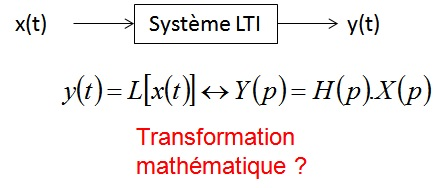
\includegraphics[scale=0.5]{images/Position_Pb_Laplace.jpg}
		\caption{Lien entre la réponse impulsionnelle et la fonction de transfert}	
		\label{Fig:Position_Pb_Laplace} 
	\end{figure}
	
	 La transformée de Laplace permet de passer du domaine temporel à son domaine dual, le domaine fréquentiel. Dans les chapitres suivants, nous présenterons un autre type de transformation dérivée de la transformée de Laplace : la transformée de Fourier, qui sera très utile pour l'analyse des signaux, ainsi que pour l'étude des systèmes en régime permanent.
	
	\vspace{0.5\baselineskip}
	\underline{Remarque :}
	Dans ce chapitre, on ne considère que des fonctions causales. L'instant d'apparition des signaux se fera en t = 0. Pour représenter cette condition, l'ensemble des signaux en entrée et en sortie que nous allons considérer seront multiplier par l'échelon de Heaviside u(t).
	\vspace{1\baselineskip}
	
	\section{Transformation d'une fonction temporelle au domaine fréquentiel}
	Dans le domaine temporel, l'entrée et la sortie du système sont reliées par la réponse impulsionnelle h(t) et le produit de convolution. Cela est vrai quel que soit le type d'excitation appliquée en entrée du système. Le passage dans le domaine fréquentiel suppose une excitation exponentielle complexe. Considérons ce cas dans le domaine temporel : la réponse sera donc égale au produit de convolution entre la réponse impulsionnelle et l'excitation exponentielle complexe. Nous considérons dans un premier temps un signal défini sur tout le domaine temporel. Elle peut être modifiée selon la forme donnée par l'équation \ref{Demo_Laplace}.
	
	\begin{equation}\label{}
	y(t) = h*x(t) = h * exp(pt) = \int_{-\infty}^{+\infty} h(\tau) \cdot exp(p(t-\tau))
 \deriv \tau 	
 	\end{equation}
	\begin{equation}\label{Demo_Laplace}
	y(t) = exp(pt) \int_{-\infty}^{+\infty} h(\tau) \cdot exp(-p\tau)
	\deriv \tau 	
	\end{equation}
	
	On remarque que la réponse du système est le produit entre l'excitation et un terme intégrale dépendant de la réponse impulsionnelle. On retrouve donc une forme très similaire à celle vue à l'équation \ref{Def_fonction_tranfert}, reliant réponse et excitation exponentielle complexe, via la fonction de transfert. Ce terme intégrale n'est donc rien d'autre que la réponse du système LTI dans le domaine fréquentiel complexe, c'est-à-dire sa fonction de transfert.
	\begin{figure}[h!]
		\centering
		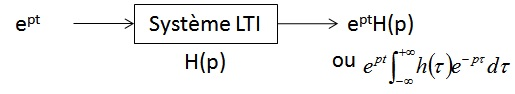
\includegraphics[scale=0.7]{images/LTI_Laplace.jpg}
		\caption{Lien via la transformée de Laplace entre l'excitation exponentielle complexe et la réponse d'un système LTI}	
		\label{Fig:LTI_Laplace} 
	\end{figure}
	
	Nous venons de mettre en évidence une transformation mathématique permettant de passer de la représentation temporelle d'une fonction à sa représentation fréquentielle complexe. Cette transformée s'appelle la transformée de Laplace. Elle est donnée par \ref{Fonction_Transfert_Laplace_non_causale} dans le cas général.
	\begin{equation}\label{Fonction_Transfert_Laplace_non_causale}
	H(p) = \int_{-\infty}^{+\infty} h(t) \cdot exp(-pt)	\deriv t~,~~p \in \mathbb{C}	
	\end{equation}	
	
	La démonstration précédente reste valable dans le cas d'un signal causal, défini pour t > 0. Dans ce cas, on peut écrire :
	\begin{equation}\label{Fonction_Transfert_Laplace_causale}
	H(p) = \int_{0}^{+\infty} h(t) \cdot exp(-pt)	\deriv t~,~~p \in \mathbb{C}	
	\end{equation}
	
	\textbf{\underline{Remarque :}}
	On vient aussi de montrer que la fonction de transfert, exprimée dans le domaine des fréquences complexes p, n'est rien d'autre que la transformée de Laplace de la réponse impulsionnelle.\\
	
	\section{Transformée de Laplace}
	\subsection{Définition}
	La transformée de Laplace est une transformation mathématique, transformant une fonction temporelle en une fonction définie dans le domaine des fréquences complexes p. Nous noterons $\mathcal{L}$ cette transformation. On distingue deux types de transformée de Laplace : bilatérale (\ref{Transfo_Laplace_non_causale}) et unilatérale (\ref{Transfo_Laplace_causale}). Cette dernière s'impose naturellement dès que l'on considère des systèmes causaux (h(t) = 0 pour t <0). Dans la suite, comme nous ne traiterons que de systèmes causaux, nous ne considérerons que la transformée de Laplace unilatérale.
	\begin{equation}\label{Transfo_Laplace_non_causale}
	F(p) = \mathcal{L}[f(t)] = \int_{-\infty}^{+\infty} f(t) \cdot exp(-pt)	\deriv t~,~~p=\sigma + j \omega	
	\end{equation}
	\begin{equation}\label{Transfo_Laplace_causale}
	F(p) = \mathcal{L}[f(t)] = \int_{0^{+}}^{+\infty} f(t) \cdot exp(-pt)	\deriv t~,~~p=\sigma + j \omega	
	\end{equation}
	
	\underline{\textbf{Opérateur de Heaviside s :}}\\
	Dans la littérature scientifique anglo-saxonne, lorsque la transformée de Laplace est utilisée, l'opérateur p, représentant les fréquences complexes, apparait rarement. Il est remplacé par un opérateur noté "s" et appelé opérateur de Heaviside en hommage à Oliver Heaviside. Il est l'inventeur des méthodes mathématiques de résolution des équations différentielles pour les circuits électroniques, équivalentes à la transformée de Laplace.\\
	
	

	
	\subsection{Conditions d'existence de la transformée de Laplace et stabilité des systèmes}
	Il est important de noter que la transformée de Laplace n'existe que si l'intégrale converge. Ceci n'est pas le cas pour toutes les valeurs de p.
	L'objectif de ce cours n'est pas de faire ce calcul intégrale, mais plutôt de l'utiliser comme outil pour l'étude des systèmes linéaires. Nous utiliserons la plupart du temps des tables contenant les transformées pour les fonctions les plus courantes. Néanmoins, nous allons mettre en œuvre ce calcul à travers un exemple et indiquer les conditions d'existence de la transformée de Laplace. Nous allons mettre en évidence ce que cela signifie du point de vue de la stabilité des systèmes LTI. Par souci de simplification, on dira qu'un système est stable s'il converge vers une valeur finie.
	Exemple : considérons un système LTI dont la réponse impulsionnelle est définie par la fonction : $h(t) = exp(\alpha t)u(t) $ où $\alpha$ est un réel quelconque.
	Calculons sa transformée de Laplace à l'aide de l'équation \ref{Transfo_Laplace_non_causale} :
	\begin{equation*}
	H(p) = \mathcal{L}[exp(\alpha t)u(t)] = \int_{-\infty}^{+\infty}exp(\alpha t)u(t) \cdot exp(-pt) \deriv t
	\end{equation*}
	\begin{equation*}
	H(p) = \int_{0}^{+\infty}exp(-(p-\alpha) t) \deriv t
	\end{equation*}
	\begin{equation*}
	H(p) = \lim_{T \to +\infty} \frac{1-exp(-(p-\alpha)T)}{p-\alpha} = \lim_{T \to +\infty} \frac{1-exp(-(\sigma-\alpha)T)exp(-j\omega T)}{p-\alpha}
	\end{equation*}
	La transformée de Laplace existera si cette intégrale converge. Cela dépend uniquement de la partie réelle $\sigma$ de la fréquence complexe :
	\begin{equation}\label{}
	F(p) = \left \{
	\begin{array}{l l}
	\frac{1}{p-\alpha}  & si~\sigma>\alpha \\
	\infty   & sinon \\
	\end{array}
	\right .	 	
	\end{equation}
	
	Si on représente l'excitation en fréquence dans le plan P, il existe un
	domaine d'existence de la transformée de Laplace appelé domaine de
	convergence. Il s'agit d'un plan où Re(p) = $\sigma $ \textgreater{} $\alpha $. Nous le
	représentons dans deux cas différents :  $\alpha $ \textless{} 0 et  $\alpha $
	\textgreater{} 0, et allons analyser sa signification concrète.
	\begin{figure}[h!]
		\centering
		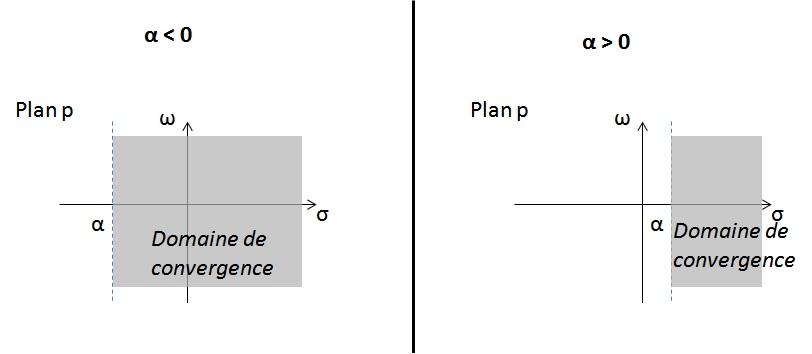
\includegraphics[scale=0.8]{images/Domaine_convergence_exp_at.jpg}
		\caption{Domaine de convergence de la fonction $exp(\alpha t)$}	
		\label{Fig:Domaine_convergence_exp_at} 
	\end{figure}
	Le domaine de convergence indique, dans le cas d'une excitation
	exponentielle complexe, l'ensemble des fréquences complexes pour lequel
	le système convergera. Pour s'en
	convaincre, considérons une excitation exponentielle, de fréquence
	complexe $p_{0} =  \beta +j \omega $. Reprenons la forme initiale dérivée de la réponse	impulsionnelle.
	\begin{equation*}
	y(t) = exp(p_{0}t)\int_{-\infty}^{+\infty}h(\tau)exp(-p_{0}\tau) \deriv \tau 
	\end{equation*}
	\begin{equation*}
	y(t) = exp((\beta+j\omega)t)\int_{-\infty}^{+\infty}exp(\alpha \tau)exp(-(\beta+j\omega)\tau) \deriv \tau 
	\end{equation*}
	\begin{equation*}
	y(t) = exp((\beta+j\omega)t)\int_{-\infty}^{+\infty}exp(-(\beta-\alpha+j\omega)\tau) \deriv \tau 
	\end{equation*}
	\begin{equation}
	y(t) = \lim_{T \to +\infty} \frac{exp((\beta+j\omega)t)(exp(-(\beta-\alpha+j\omega)T)-1)}{\beta-\alpha+j\omega} 
	\end{equation}
	Cette fonction converge si la partie réelle $\beta $ de la fréquence de
	l'excitation est supérieure à  $\alpha $, autrement dit si la fréquence complexe
	d'excitation appartient au domaine de convergence, mais aussi si $\beta $
	\textless{} 0. Dans le cas contraire, le signal d'entrée va diverger pour
	t \textgreater{} 0. Cette double condition sur $\beta $ n'est possible que si $\alpha $
	\textless{} 0, qui est donc une condition nécessaire pour garantir la stabilité du système.\\
	
	\textbf{\underline{Cas d'une excitation harmonique :}}
	
	Cette situation correspond au cas où $\beta $ = 0. Le système sera stable
	uniquement si, dans le plan p, l'axe des imaginaires appartient au
	domaine de convergence. Dans le chapitre consacré à la transformée de
	Fourier, nous verrons qu'elle est équivalente à une transformée de
	Laplace, mais pour une fréquence purement complexe $\beta $ = 0. Si l'axe des
	imaginaires appartient au domaine de convergence, alors la transformée
	de Fourier de la fonction pourra exister.\\
	
	\subsection{Pôles et zéros d'une fonction de transfert}
	
	Reprenons l'exemple précédent. Comme nous l'avions introduit dans le
	chapitre précédent, $\alpha $ correspond à un pôle de la réponse du système. Sa
	stabilité est liée à sa partie réelle.~
	
	Toutes les transformées de Laplace que l'on considère peuvent se mettre sous la forme d'une fonction rationnelle, où le numérateur N(p) et dénominateur D(p) sont
	des polynômes. Eux-mêmes peuvent être exprimés en fonction de leurs
	racines appelés zéros et pôles respectivement. Ceux-ci correspondent à
	des fréquences complexes particulières qui :
	\begin{itemize}
		\item annulent la fonction de transfert dans le cas des zéros p\textsubscript{zi}
	
		\item font tendre la fonction de transfert vers l'infini dans le cas des pôles p\textsubscript{pj}
	\end{itemize}
	
	\begin{equation}\label{key}
	F(p) = \frac{N(p)}{D(p)} = \frac{b_{m}p^{m}+...+b_{1}p+b_{0}}{a_{n}p^{n}+...+a_{1}p+a_{0}} ~\Rightarrow ~ F(p) = G \frac{\prod_{i=1}^{m}(p-p_{zi})}{\prod_{i=1}^{n}(p-p_{pj})}
	\end{equation}
	où G est le gain de la fonction de transfert.
	Comme nous l'avions déjà vu dans le chapitre 2, la position des pôles nous donne une indication sur l'allure temporelle de la fonction de transfert (réponse naturelle).
	Quel que soit le système linéaire considéré, la position de ces pôles va déterminer la stabilité du système. Vous approfondirez ces concepts dans le cours d'automatique.
	
	\section{Propriétés de la transformée de Laplace}
	Dans cette partie, nous allons passer en revue plusieurs des propriétés importantes de la transformée de Laplace, qui facilitent les calculs de la transformée de Laplace et les applications associées. Nous ne démontrerons pas l'ensemble de ces propriétés.
	\subsection{Linéarité}
	La transformée de Laplace est linéaire. La transformée de Laplace d'une somme pondérée de fonction est la somme des transformées de Laplace individuelle de ces fonctions, pondérées de la même manière. Elle vérifie donc la relation suivante :
	\begin{equation}\label{key}
	a \cdot f(t)+b \cdot g(t) \longleftrightarrow a \cdot F(p)+b \cdot G(p)~~,~avec~F(p)=\mathcal{L}[f(t)]~et~G(p)=\mathcal{L}[g(t)]
	\end{equation}
	
	\subsection{Théorème du retard}
	
	Supposons que l'on connaisse la transformée de Laplace F(p) de la
	fonction causale f(t), qui est nulle pour t \textless{} 0. Si on a
	retardé de t\textsubscript{0} cette fonction, elle devient
	f(t-t\textsubscript{0}) et s'annule pour tout t \textless{}
	t\textsubscript{0}. Calculons sa transformée de Laplace à partir de (\ref{Transfo_Laplace_causale})
	et appliquons le changement de variable w = t-t\textsubscript{0}. On
	montre que la transformée de Laplace de la fonction retardée est la
	transformée de Laplace non retardée multipliée par $e^{-pt_{0}}$.
	
	\begin{equation*}
	F_{t0}(p) = \mathcal{L}[f(t-t_{0})]=\int_{t_{0}}^{+\infty}f(t-t_{0})exp(-pt) \deriv t   
	\end{equation*}
	\begin{equation*}
	F_{t0}(p) = \int_{0}^{+\infty}f(w)exp(-p(w+t_{0})) \deriv w = \int_{0}^{+\infty}f(w)exp(-pw)exp(-pt_{0}) \deriv w  
	\end{equation*}
	\begin{equation}\label{}
	F_{t0}(p) = F(p)\cdot exp(-pt_{0})
	\end{equation}
	
	\subsection{Théorème du changement d'échelle}
	
	Supposons que l'on connaisse la transformée de Laplace F(p) de la
	fonction causale f(t). Dilatons l'échelle de temps de cette fonction par
	un facteur réel k. La fonction devient f(kt). Calculons la transformée
	de Laplace de cette version dilatée de f(t), en appliquant le changement
	de variable $w = kt$.
	\begin{equation*}
	F_{k}(p) = \mathcal{L}[f(kt)]=\int_{t_{0}}^{+\infty}f(kt)exp(-pt) \deriv t  =\int_{t_{0}}^{+\infty}\frac{1}{k}f(w)exp(-\frac{p}{k}w) \deriv w 
	\end{equation*}
	\begin{equation}\label{}
	F_{k}(p) = \frac{1}{k}\cdot F(\frac{p}{k})
	\end{equation}
	
	
	\subsection{Translation dans le domaine fréquentiel}
	Un décalage d'une valeur $p_{1}$ dans le domaine de Laplace conduit à une multiplication par $e^{p_{1}t}$ dans le domaine temporel.
	\begin{equation}\label{key}
		soit~F(p)=\mathcal{L}[f(t)]~alors~\mathcal{L}[e^{p_{1}t}f(t)] = F(p-p_{1})	
	\end{equation}
	
	Dans le domaine fréquentiel ($\alpha$ = 0), cela est équivalent à une translation du spectre. Ce procédé est bien connu en télécommunication, car il est utilisé pour moduler les signaux à transmettre.
	
	
	
	\subsection{Dérivation dans le domaine temporel}
	Considérons le cas d'une fonction f(t) continue non nulle pour t > 0. La transformée de Laplace de la dérivée de cette fonction est donnée par :
	
	\begin{equation}\label{key}
	\mathcal{L}[\frac{df}{dt}] = p\cdot F(p)-f(0^{+}) ~~~avec~f(0^{+})=\lim_{t\rightarrow0^{+}}f(t)
	\end{equation}

	On remarque que l'opérateur dérivée correspond à une multiplication de
	la transformée de Laplace par p. Cependant, il est nécessaire de tenir
	compte de la condition initiale f(0\textsuperscript{+}).
	
	Il est possible de généraliser cette relation au cas où l'on dérive N
	fois la fonction. L'expression devient :
	\begin{equation}\label{key}
	\mathcal{L}[\frac{d^{n}f}{dt^{n}}] = p^{n}\cdot F(p)-p^{n-1}\cdot f(0^{+})-p^{n-2}\cdot \frac{df}{dt}(0^{+})-...-p\frac{d^{n-2}f}{dt^{n-2}}(0^{+})-\frac{d^{n-1}f}{dt^{n-1}}(0^{+})
	\end{equation}
	Le calcul nécessite de connaître les conditions initiales non seulement sur la valeur de la fonction mais aussi pour ses (n-1) premières dérivées.
	
	\subsection{Dérivation dans le domaine des fréquences complexes p}
	Dériver une fonction dans le domaine de Laplace revient à multiplier cette fonction par -t dans le domaine temporel.
	\begin{equation}\label{key}
		soit~F(p)=\mathcal{L}[f(t)]~alors~\mathcal{L}[-t\cdot f(t)] = \frac{dF(p)}{dp})
	\end{equation}
	
	Cette propriété peut se généraliser au cas où l'on dérive N fois la fonction dans le domaine de Laplace, qui revient à multiplier la fonction temporelle par le terme $(-t)^{N}$.
	\begin{equation}\label{key}
	soit~F(p)=\mathcal{L}[f(t)]~alors~\mathcal{L}[-(t)^{n}\cdot f(t)] = \frac{dF^{n}(p)}{dp^{n}})
	\end{equation}
	
	
	\subsection{Intégration temporelle}
	Considérons le cas d'une fonction f(t) continue non nulle pour t > 0. La transformée de Laplace de son intégrale de 0 à t est donnée par :
	\begin{equation}\label{key}
		soit~F(p)=\mathcal{L}[f(t)]~alors~\mathcal{L}[\int_{0}^{t}f(\tau)d\tau]=\frac{F(p)}{p}	
	\end{equation}
	
	Cette propriété peut s'étendre au cas où on intègre N fois la fonction temporelle :
	
	\begin{equation}\label{key}
	soit~F(p)=\mathcal{L}[f(t)]~alors~\mathcal{L}[\int ... \int_{0}^{t}f(\tau)d\tau]=\frac{F(p)}{p^{n}}	
	\end{equation}
	

	\subsection{Théorème de la valeur initiale}
	
	On considère une fonction f(t) continue non nulle pour t > 0. On peut montrer que :
	\begin{equation}\label{key}
		\lim_{t \to 0^{+}}f(t) = \lim_{p \to +\infty}pF(p)
	\end{equation}
	
	
	\subsection{Théorème de la valeur finale}
	De la même manière, on peut montrer que la fonction f(t) tend de manière asymptotique vers la valeur suivante :
	\begin{equation}\label{key}
		\lim_{t \to +\infty}f(t) = \lim_{p \to 0}pF(p)
	\end{equation}
	
	Cette propriété, couplée à celle de l'intégration temporelle, permet aussi de calculer l'aire sous la courbe temporelle entre 0 et une valeur t > 0 :
	\begin{equation}\label{key}
		\int_{0^{-}}^{t}f(t)dt=F(0)
	\end{equation}
	
	\subsection{Multiplication et produit de convolution}
	Multiplication et produit de convolution (\ref{Demo_produit_convolution}) sont deux opérations complémentaires dans les domaines temporelles et de Laplace. On peut ainsi écrire les deux propriétés suivantes :
	\begin{equation}\label{key}
		\mathcal{L}[f(t)\cdot g(t)] = F*G(p)
	\end{equation}
	\begin{equation}\label{key}
	\mathcal{L}[f*g(t)] = F(p) \cdot G(p)
	\end{equation}
	
	Avec cette dernière propriété, on retrouve la relation vue entre la fonction de transfert et la réponse impulsionnelle. Dans le domaine temporel, la réponse d'un système correspond au produit de convolution entre l'excitation et la réponse impulsionnelle. Avec une excitation exponentielle complexe, cette relation est équivalente au produit entre l'excitation exprimée dans le domaine de Laplace et la fonction de transfert, soit la transformée de Laplace de la réponse impulsionnelle.
	
	\subsection{Fonctions causales avec N répétitions}
	On considère une fonction $f_{1}(t)$, dite génératrice, que l'on répète N fois de manière périodique pour former une nouvelle fonction causale f(t). La période est notée T. La fonction f(t) s'écrit :
	\begin{equation*}
	f(t)=\sum_{k=0}^{N-1}f_{1}(t-kT)
	\end{equation*}
	
	On note $F_{1}(p)$ la transformée de Laplace de la fonction génératrice. A partir du théorème du retard, on peut calculer la transformée de Laplace de la somme des N termes précédents.
	\begin{equation*}
	F(p)=\mathcal{L}[f(t)]=F_{1}(p)(1+e^{-Tp}+e^{-2Tp}+...+e^{-(N-1)Tp})
	\end{equation*}
	On retrouve une série de N termes exponentiels mis à la puissance k, qui peut se simplifier selon la relation ci-dessous. 
	\begin{equation}
	F(p)=\mathcal{L}[f(t)]=F_{1}(p)\frac{1-e^{-(N-1)Tp}}{1-e^{-Tp}}
	\end{equation}
	
	
	\subsection{Fonctions périodiques causales}
	La propriété précédente peut être réutilisée pour déterminer la transformée de Laplace d'une fonction causale périodique, de période T et générée à partir d'une fonction génératrice $f_{1}(t)$. La fonction périodique s'écrit : $f(t)=\sum_{k=0}^{+\infty}f_{1}(t-kT)$.
	
	On en déduit la transformée de Laplace de la fonction en remarquant que $|e^{-kTp}| < 1$ car la partie réelle de p est positive pour garantir la convergence.
	\begin{equation}
	F(p)=\mathcal{L}[f(t)]=\lim_{N \to +\infty}F_{1}(p)\frac{1-e^{-(N-1)Tp}}{1-e^{-Tp}}=F_{1}(p)\frac{1}{1-e^{-Tp}}
	\end{equation}
	
	Toute fonction exprimée dans le domaine de Laplace où apparaît le terme $\frac{1}{1-e^{-Tp}}$ correspond à la transformée de Laplace d'une fonction périodique de période T.
	
	\vspace{1\baselineskip}
		
	
	\section{Transformée de Laplace des fonctions courantes}
	Le tableau \ref{Tab:Transfo_Laplace_usuelle} donne la transformée de Laplace des fonctions causales les plus courantes, et pour lesquelles des formes mathématiques simples existent. Pour la plupart, aucune démonstration n'est donnée, mais les transformées peuvent être retrouvées. Nous nous limiterons à deux exemples de mise en forme de la transformée de Laplace pour deux formes temporelles courantes, sachant que nous avons déjà vu celle d'une fonction exponentielle.\\
	
	\underline{Exemple 1 :} échelon unitaire f(t) = u(t)
	\begin{equation*}
	F(p)=\mathcal{L}[u(t)] = \int_{-\infty}^{+\infty}u(t)exp(-pt) \deriv t =\int_{0}^{+\infty}exp(-pt) \deriv t = [-\frac{exp(pt)}{p}]_{0}^{+\infty}=\frac{1}{p}
	\end{equation*}
	
	\underline{Exemple 2 :} fonction cosinusoïdale
	\begin{equation*}
	f(t)=cos(\omega t)u(t)
	\end{equation*}
	\begin{equation*}
	F(p)=\mathcal{L}[f(t)]=\int_{-\infty}^{+\infty}cos(\omega t)u(t) \deriv t=\int_{0}^{+\infty}\frac{exp(j\omega t)+exp(-j\omega t)}{2} \deriv t
	\end{equation*}
	\begin{equation*}
	F(p)=\frac{1}{2}\int_{0}^{+\infty}(exp((j\omega-p) t)+exp(-(j\omega+p) t)) \deriv t=\frac{1}{2}([\frac{exp((j\omega-p) t)}{j\omega-p}]_{0}^{+\infty}-[\frac{exp((j\omega-p) t)}{j\omega-p}]_{0}^{+\infty})
	\end{equation*}
	\begin{equation}\label{}
	F(p)=\frac{1}{2}(-\frac{1}{j\omega-p}+\frac{1}{j\omega+p})=\frac{p}{p^{2}+\omega^{2}}
	\end{equation}
	
	\underline{Tableau récapitulatif des transformées de Laplace :}
	
	\begin{table}[h!]
		\centering
		\caption{\label{Tab:Transfo_Laplace_usuelle} Tableau récapitulatif des transformées de Laplace usuelles}
		\begin{tabular}{|l|c|}
			\hline
			\textbf{Fonctions temporelles f(t)} & \textbf{Transformée de Laplace F(p)} \\
			\hline
			Echelon unitaire u(t) & $\frac{1}{p}$ \\	
			\hline
			Fonction rampe $f(t)=t\cdot u(t)$ & $\frac{1}{p^{2}}$ \\	
			\hline
			Fonction rampe polynomiale $f(t)=\frac{t^{n-1}}{(n-1)!} u(t)$ & $\frac{1}{p^{n}}$ \\	
			\hline
			Fonction exponentielle $f(t)=e^{-\alpha t} u(t)$ & $\frac{1}{p+\alpha}$ \\	
			\hline
			$f(t)=te^{-\alpha t} u(t)$ & $\frac{1}{(p+\alpha)^{2}}$ \\
			\hline
			$f(t)=\frac{t^{n-1}}{(n-1)!}e^{-\alpha t} u(t)$ & $\frac{1}{(p+\alpha)^{n}}$ \\
			\hline
			Fonction cosinus $f(t)=cos(\omega t)u(t)$ & $\frac{p}{p^{2}+\omega^{2}}$ \\
			\hline
			Fonction sinus $f(t)=sin(\omega t)u(t)$ & $\frac{\omega}{p^{2}+\omega^{2}}$ \\
			\hline
			Fonction cosinus amorti $f(t)=e^{-\alpha t}cos(\omega t)u(t)$ &  $\frac{p+\alpha}{(p+\alpha)^{2}+\omega^{2}}$ \\
			\hline
			Fonction rampe limitée $f(t)= \left\{\begin{array}{l}
			A\frac{t}{\tau}u(t)~,~si~t \leq \tau \\
			A\cdot u(t) \\
			\end{array} 
			\right . $ & $A\frac{1-e^{-p\tau}}{p^{2}\tau}$ \\
			\hline
		\end{tabular}	
	\end{table}


	A partir de cette table, il est possible de dériver les transformées de Laplace pour d'autres fonctions temporelles. En effet, il suffit d'identifier des formes dont la transformée de Laplace est connue et utiliser les différentes propriétés de la transformée pour en déduire l'expression de la transformée de Laplace.
	
	\vspace{1\baselineskip}
	
	\textbf{\underline{Exemple : }}
	
	\begin{minipage}[l]{0.6\linewidth}
		Soit la fonction temporelle f(t) dont l'évolution temporelle est présentée ci-contre. Déterminez la transformée de Laplace de cette fonction.	
	\end{minipage} \hfill
	\begin{minipage}[r]{0.6\linewidth}
		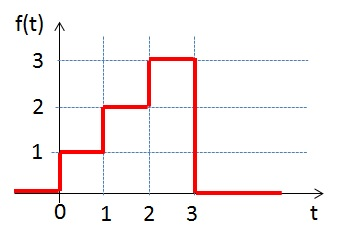
\includegraphics[scale=0.7]{images/Ex_Laplace_Fonction_marche_escalier.jpg} 	
	\end{minipage}
	\vspace{0.5\baselineskip}
	
	La fonction discontinue ci-dessus peut être exprimée sous la forme d'une somme de fonctions échelons. En repérant les instants de transition et les amplitudes des paliers, celle-ci s'écrit : $f(t)= u(t) + u(t-1) + u(t-2) - 3u(t-3)$.
	La transformée de Laplace étant linéaire, la transformée de Laplace de f(t) sera la somme des transformées de chaque terme de l'expression de f(t). En identifiant la transformée de Laplace de la fonction échelon et en appliquant le théorème du retard, on détermine l'expression de la transformée de Laplace de f(t) :
	\begin{equation*}
	F(p)=\mathcal{L}[f(t)]=\mathcal{L}[u(t)]+\mathcal{L}[u(t-1)]+\mathcal{L}[u(t-2)]-3\mathcal{L}[u(t-3)]
	\end{equation*}
	\begin{equation*}
	F(p)=\frac{1}{p}+\frac{e^{-p}}{p}+\frac{e^{-2p}}{p}-3\frac{e^{-3p}}{p}
	\end{equation*}
	\vspace{1\baselineskip}
		
	
	
	\section{Transformée de Laplace inverse}
	
	
	Du point de vue pratique, le but de la transformée de Laplace est de fournir un outil simple pour le calcul des réponses temporelles des systèmes linéaires. Elle permet de calculer la représentation fréquentielle d'une fonction à partir de sa représentation dans le domaine temporel. Dans le domaine fréquentiel, le calcul de la réponse du système est facilité en passant par la fonction de transfert. Cependant, si nous ne disposons pas d'une transformation mathématique permettant de réaliser le passage inverse, cette approche perd de son intérêt.  Fort heureusement, cet outil existe. Il s'agit de la transformée de Laplace inverse, que nous allons rapidement présenter. 
	 Elle permet de transformer une fonction définie dans le domaine des fréquences complexes p en une fonction définie dans le domaine temporel. Nous la noterons $\mathcal{L}^{-1}$. Comme la transformée de Laplace, la transformée de Laplace inverse est une fonction linéaire.
	
	
	\subsection{Méthode pratique d'utilisation}
	
	La transformée de Laplace inverse est donnée par la formule de Bromwich-Mellin , où $\sigma$ est choisi pour que l'intégrale converge.
	
	\begin{equation}\label{TL_inverse}
	f(t) = \mathcal{L}^{-1}[F(p)]=\frac{1}{2\pi j}\int_{\sigma - j\infty}^{\sigma + j\infty}F(p)exp(pt) \deriv p
	\end{equation}
	
	Dans la pratique, cette formule est difficile à mettre en œuvre car elle nécessite de calculer une intégrale dans le plan complexe. Ceci dépasse le cadre de ce cours et nous n'effectuerons pas de calcul de cette transformée. Dans ce cours, nous privilégierons la méthode utilisée en pratique, basée sur les tables reliant des fonctions courantes et leur transformée de Laplace, comme le tableau \ref{Tab:Transfo_Laplace_usuelle}. Il s'agit de rechercher des paires de transformées. A partir de la fonction F(p), on identifie des fonctions connues et on déduit la fonction temporelle correspondante. Dans le cas de fonctions compliquées, le calcul de la forme temporelle passe par des approches basées sur le calcul numérique, non détaillées ici. Dans de nombreux cas pratiques, les expressions des transformées de Laplace peuvent être données sous la forme d'une fraction rationnelle, pour laquelle on ne dispose pas directement de la fonction temporelle correspondante. Il est nécessaire de transformer d'abord l'expression de la transformée de Laplace avant d'identifier des formes courantes. On utilisera notamment une technique de décomposition en pôles et en résidus.
	 
	\subsection{Décomposition pôles-résidus}
	Comme nous l'avons dans la partie II.3, la plupart des transformées de Laplace peuvent être mises sous la forme d'une fonction rationnelle, rapport de deux polynômes faisant apparaitre leurs racines (pôles et zéros). Cependant, il n'existe sans doute pas une paire de transformées simples pour toutes les fonctions rationnelles. Pour appliquer la méthode précédente, il est nécessaire de décomposer cette fonction rationnelle en éléments plus simples, dont on connait la paire de transformées.
	Il est possible de montrer que toute fonction rationnelle de deux polynômes peut s'écrire sous la forme d'une somme d'éléments simples, appelées fractions partielles ne dépendant que des pôles et de constantes appelées résidus. Cette décomposition s'appelle la décomposition pôles-résidus, dont la forme est illustrée par \ref{Forme_decompo_pole_residu}. Cette décomposition ne fonctionne qu'avec des fractions dites "propres" pour lesquelles le nombre n de pôles est supérieur ou égal au nombre m de zéros. Dans ce cas, la fraction rationnelle peut se décomposer en n termes dont il faut déterminer les résidus $A_{n}$.
	
	\begin{equation}\label{Forme_decompo_pole_residu}
	F(p)=\frac{N(p)}{D(p)}=A\frac{(p-p_{zm})...(p-p_{z1})}{(p-p_{pn})...(p-p_{p1})}=\frac{A_{1}}{p-p_{p1}}+\frac{A_{2}}{p-p_{p2}}+...+\frac{A_{n}}{p-p_{pn}}
	\end{equation}
	
	On voit immédiatement l'intérêt de cette approche car on remarque qu'on identifie immédiatement la paire de transformée simple. En effet, la transformée de Laplace inverse de la fraction partielle est une fonction exponentielle, dépendante du pôle.
	
	\vspace{0.5\baselineskip}
	
	\textbf{\underline{Cas d'une fraction impropre (n < m) :}}
	
	Avant de voir comment réaliser cette décomposition pôles-résidus, traitons d'abord le cas des fractions impropres (plus de zéros que de pôles). La décomposition pôles-résidus n'est pas directe. Il est cependant possible d'exprimer cette fraction impropre comme la somme d'un terme (qui ne sera pas une fraction) et d'une fraction propre (\ref{reduction_fraction_impropre}). Il est indispensable que le premier terme ait une transformée de Laplace inverse connue.
	\begin{equation}\label{reduction_fraction_impropre}
	\frac{N(p)}{D(p)}=Q(p)+\frac{R(p)}{D(p)}~,~si~n<m
	\end{equation}
	
	 Q(p) n'est rien d'autre que le quotient de la division entre N(p) et D(p), tandis que R(p) est le reste. Cette décomposition consiste donc à faire une division entre deux polynômes. Illustrons-le par un exemple.
	 
	 \vspace{0.5\baselineskip}
	 \underline{Exemple :} décomposer la fonction $\frac{2p^{3}+p^{2}-4p}{p^{2}+p-2}$ pour faire apparaître une fraction propre.
	 
	 La division est décrite ci-dessous. Elle s'effectue comme suit : on identifie chaque terme du quotient afin d'éliminer le terme de plus haut degré du numérateur. Par exemple, le terme de plus haut degré de Q(p), 2p, est choisi de manière à éliminer $2p^{3}$ du numérateur. Comme il ne reste plus que $p^{2}$, le prochain terme de Q(p) est -1. Le calcul s'arrête ensuite. On a déterminé Q(p) et R(p).
	 
	 \begin{figure}[h!]
	 	\centering
	 	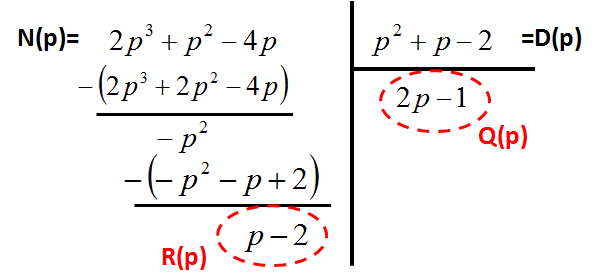
\includegraphics[scale=0.5]{images/ex_fraction_impropre.png} 
	 \end{figure}
 	
 	On peut donc écrire $\frac{2p^{3}+p^{2}-4p}{p^{2}+p-2}=(2p-1)+\frac{p-2}{p^{2}+p-2}=Q(p)+\frac{R(p)}{D(p)}$. Le terme $\frac{R(p)}{D(p)}$ est une fraction propre, tandis qu'on peut associer à Q(p) une transformée de Fourier simple, en l'occurence $2tu(t)-\delta(t)$ (voir tableau \ref{Tab:Transfo_Laplace_usuelle}). \\
	
	
	Nous considérons maintenant que nous disposons d'une fraction propre. Voyons comment effectuer facilement la décomposition pôles-résidus. Un préalable consiste à disposer des zéros et des pôles de la fonction rationnelle, afin de pouvoir écrire l'égalité de l'équation \ref{reduction_fraction_impropre}. Il existe plusieurs méthodes de décomposition pôles-résidus, nous n'en mentionnerons que deux. 
	
	\subsubsection{Association des fractions partielles}
	La première méthode consiste à partir de la forme en fractions partielles, puis de les associer pour revenir à la forme initiale de la fonction rationnelle, mais exprimée avec les résidus. On obtient ainsi n équations où les n inconnues sont les résidus. Prenons l'exemple suivant, où les pôles sont égaux à 1 et -2 :
	\begin{equation*}
	\frac{p-2}{p^{2}+p-2}=\frac{A}{p-1}+\frac{B}{p+2}
	\end{equation*}
	On cherche les résidus A et B. En les associant, on obtient $\frac{p-2}{p^{2}+p-2}=\frac{A(p+2)+B(p-1)}{p^{2}+p-2}=\frac{(A+B)p+(2A-B)}{p^{2}+p-2}$. On détermine les résidus en résolvant le système d'équations suivants :
	\begin{equation*}
	\left \{
	\begin{array}{l l}
	A+B=1 \\
	2A-B=-2 \\
	\end{array}
	\right .
	\end{equation*}
	On trouve les solutions suivantes : $A=-\frac{1}{3}$ et $B=\frac{4}{3}$. Cette approche simple peut devenir fastidieuse lorsque le nombre de pôles s'accroit. 
	
	\subsubsection{Méthode du cache}
	
	Une méthode alternative est la méthode du cache. Elle consiste à annuler un pôle pour déterminer le résidu associé, et répéter l'opération pour chaque pôle. Par exemple, supposons que l'on cherche le résidu $A_{i}$ associé au pôle $p_{pi}$. On multiplie la fraction par $(p-p_{pi})$. Dans la fraction rationnelle, l'effet du pôle va disparaitre. En prenant $p=p_{pi}$, on fera disparaitre les autres fractions partielles et on isolera ainsi le résidu $A_{i}$. Pour l'illustrer, reprenons l'exemple précédent :
	\begin{equation*}
	\frac{p-2}{p^{2}+p-2}=\frac{p-2}{(p-1)(p+2)}=\frac{A}{p-1}+\frac{B}{p+2}
	\end{equation*}
		
	Commençons par déterminer le résidu A associé au pôle p=1. On multiplie la fraction rationnelle par (p-1) et on obtient :
	\begin{equation*}
	\frac{p-2}{(p+2)}=A+\frac{B(p-1)}{p+2}
	\end{equation*}
	En fixant p = 1, on détermine $A=\frac{1-2}{(1+2)}=-\frac{1}{3}$. On répète l'opération pour déterminer l'autre résidu associé au pôle p=-2. On multiplie la fraction rationnelle par (p+2) et on obtient :
	\begin{equation*}
	\frac{p-2}{(p-1)}=\frac{A(p+2)}{p-1}+B
	\end{equation*}
	En fixant p = -2, on détermine $A=\frac{-2-2}{(-2-1)}=\frac{4}{3}$. La décomposition pôles-résidus s'écrit donc :
	\begin{equation*}
	\frac{p-2}{p^{2}+p-2}=\frac{-1}{3(p-1)}+\frac{4}{3(p+2)}
	\end{equation*}
	Sous cette forme, on identifie facilement la transformée de Laplace inverse, qui est égale à $(-\frac{1}{3}e^{t}+\frac{4}{3}e^{-2t})u(t)$.
	
	
	\vspace{1\baselineskip}
	

	
	\section{Applications} 
	Nous allons présenter deux applications où l'utilisation de la transformée de Laplace et de son inverse trouve tout leur intérêt : 
	\begin{itemize}
		\item la résolution d'équations différentielles
		\item le calcul de la réponse transitoire de systèmes linéaires
	\end{itemize}
	
	\subsection{Résolution d'équations différentielles ordinaires}
	La transformée de Laplace constitue un outil puissant de résolution des équations différentielles ordinaires, qui ne dépendent que d'une variable. De manière générale, elles peuvent s'écrire sous la forme suivante :
	\begin{equation}\label{key}
	L[t,x(t)]=f(t)
	\end{equation}
	
	où x(t) est l'inconnue, L un opérateur linéaire quelconque (superposition des effets d'opérateurs proportionnels, intégrateurs et différenciateurs) et f(t) une fonction quelconque. Dans le domaine des fréquences complexes, l'effet d'une dérivée et d'une intégration se résument à une multiplication et une division par la fréquence p. Ainsi, en passant dans le domaine fréquentiel, l'équation différentielle se transforme en une simple équation algébrique. En isolant le terme X(p) et en utilisant la transformée de Laplace inverse (à condition qu'elle existe), on pourra déterminer la solution x(t) de l'équation.
	
	\vspace{1\baselineskip}
	
	\textbf{\underline{Exemple :}} 
	
	soit l'équation différentielle suivante : $y"(t)+4y'(t)+4y(t)=0$, où y(t) est une fonction causale. On a les conditions initiales suivantes : $y(0^{+})=1$ et $y'(0^{+})=-2$. Résoudre l'équation différentielle.
	
	A l'aide du théorème de la dérivation, l'équation différentielle peut être exprimée dans le domaine de Laplace.
	\begin{equation*}
	p^{2}Y(p)-py(0^{+})-y'(0^{+})+4(pY(p)-y(0^{+}))+4Y(p)=0
	\end{equation*}
	En isolant Y(p) et en intégrant les valeurs des conditions initiales, on détermine l'expression de la solution Y(p) dans le domaine de Laplace.
	\begin{equation*}
	(p^{2}+4p+4)Y(p)=y'(0^{+})+(p+4)y(0^{+})
	\end{equation*}
	\begin{equation*}
	Y(p)=\frac{y'(0^{+})+(p+4)y(0^{+})}{p^{2}+4p+4}=\frac{p+2}{(p+2)^{2}}=\frac{1}{p+2}
	\end{equation*}
	On identifie sans difficulté la fonction temporelle associée à cette transformée de Laplace à l'aide du tableau \ref{Tab:Transfo_Laplace_usuelle}.
	\begin{equation*}
	y(t)=\mathcal{L}[Y(p)]=e^{-2t}u(t)
	\end{equation*}
	On vérifie que cette solution satisfait bien aux conditions initiales fixées et est une solution de l'équation différentielle.
	
	
	\vspace{1\baselineskip}
	
	\subsection{Calcul de la réponse transitoire d'un système linéaire}
	
	\begin{figure}[h!]
		\centering
		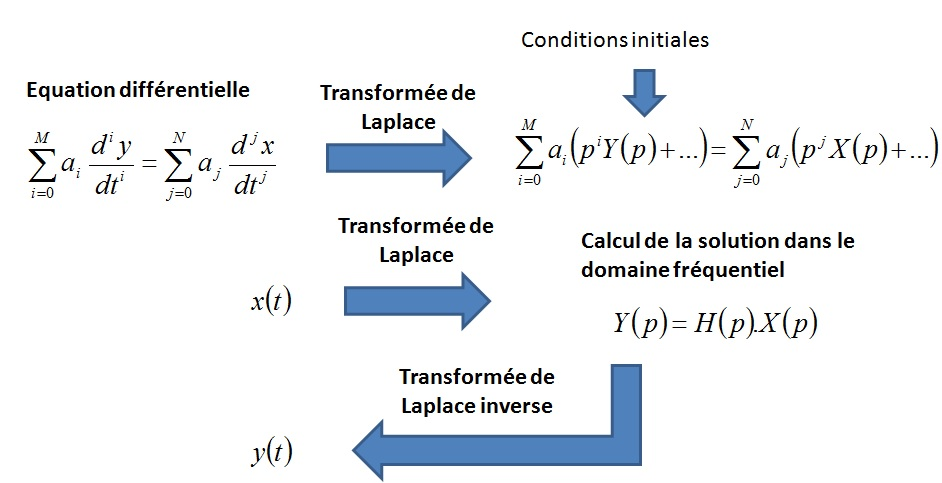
\includegraphics[scale=0.6]{images/Methodo_reso_equa_diff_Laplace.jpg}
		\caption{Méthodologie de résolution d'une équation différentielle ordinaire basée sur la transformée de Laplace}	
		\label{Fig:Methodo_reso_equa_diff_Laplace} 
	\end{figure}
	
	
	Comme nous l'avons vu avec l'équation générale du système linéaire (\ref{equation_generale_LTI}), le comportement transitoire d'un système est dicté par une équation différentielle. Déterminer la réponse temporelle à une excitation donnée revient à résoudre cette équation différentielle. Le problème est donc équivalent au précédent et la transformée de Laplace constitue encore un outil de résolution adapté à ce genre de problème. Supposons que nous disposions de la fonction de transfert H(p) du système et que l'on recherche la réponse y(t) à une excitation x(t) dont l'expression est donnée. La première étape consiste à déterminer la transformée de Laplace X(p) de l'excitation. La réponse du système dans le domaine fréquentiel Y(p) est directement le produit de la fonction de transfert et de l'excitation X(p). Ensuite, la transformée de Laplace inverse de Y(p) permet de retrouver l'expression de la réponse temporelle y(t).
	Il est bien entendu indispensable de prendre en compte les conditions initiales du système, qui vont intervenir dans la réponse naturelle du système. Si l'expression de la fonction de transfert ne les intègre pas, il est indispensable de repartir de l'équation différentielle décrivant le système et établir la fonction de transfert en intégrant l'effet des conditions initiales. La méthodologie de calcul est résumée à la figure \ref{Fig:Methodo_reso_equa_diff_Laplace}.
	
	\vspace{1\baselineskip}
	
	
	\textbf{\underline{Exemple : réponse d'un circuit RC à un échelon}}
	
	On reprend l'exemple du circuit RC (passe haut) vu dans le chapitre précédent, pour lequel nous avions calculé la réponse harmonique. Le circuit est présenté ci-dessous.
	On considère qu'il est excité par un échelon d'amplitude E en t = 0, et que le condensateur est initialement chargé (la tension initiale à ses bornes est notée $U_{C0}$). On souhaite déterminer la réponse du circuit, correspondant à la tension aux bornes de la résistance.

	\begin{figure}[h!]
	\centering
	\begin{minipage}[c]{0.4\linewidth}
		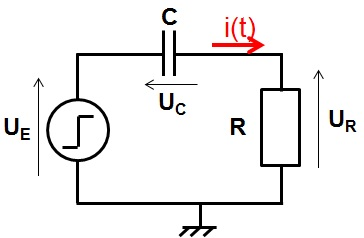
\includegraphics[scale=0.6]{images/circuit_RC_reponse_indicielle.jpg}
	\end{minipage} \hfill
	\begin{minipage}[c]{0.50\linewidth}
		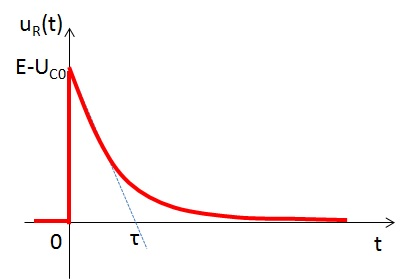
\includegraphics[scale=0.6]{images/reponse_RC_indicielle.jpg} 	
	\end{minipage}
	\caption{Circuit RC étudié (à gauche) et réponse à un échelon (à droite)}	
	\label{Fig:Circuit_RC_Laplace_inverse} 
	\end{figure}

	L'excitation du circuit s'écrit : $u_{E}(t)=Eu(t)$. Dans le domaine de Laplace, elle s'exprime : $U_{E}(p)=\frac{A}{p}$.
	Dans le chapitre précédent, nous avions déterminé l'équation différentielle liant l'excitation et la réponse du circuit. Nous allons la reprendre pour déterminer non seulement la fonction de transfert du circuit, mais aussi intégrer la condition initiale sur la charge du condensateur. On note $\tau=RC$ la constante de temps du circuit.
	\begin{equation}\label{}
	\frac{dU_{E}}{dt}=\frac{U_{R}}{RC}+\frac{dU_{R}}{dt}=\frac{U_{R}}{\tau}+\frac{dU_{R}}{dt}
	\end{equation}
	Le passage dans le domaine de Laplace de cette équation différentielle donne :
	\begin{equation*}
	pU_{E}(p)-U_{E}(0^{+})=\frac{U_{R}(t)}{\tau}+pU_{R}(p)-U_{R}(0^{+})
	\end{equation*}
	\begin{equation*}
	(p+\frac{1}{\tau})U_{R}(p)+U_{E}(0^{+})-U_{R}(0^{+})=pU_{E}(p)
	\end{equation*}
	En remarquant que $U_{E}(0^{+})-U_{R}(0^{+})$ est équivalent à la tension initiale $U_{C}(0^{+})=U_{C0}$ aux bornes du condensateur, l'équation s'écrit sous la forme ci-dessous. Le premier terme correspond à l'effet de l'excitation "filtré" par la fonction de transfert du circuit. Le second terme est lié à la présence d'une charge initiale aux bornes du condensateur.
	\begin{equation*}
	U_{R}(p) = \frac{p}{p+\frac{1}{\tau}}U_{E}(p)-\frac{1}{p+\frac{1}{\tau}}U_{C}(0^{+})=H(p)U_{E}(p)-\frac{1}{p+\frac{1}{\tau}}U_{C0}
	\end{equation*} 
	En intégrant l'expression de l'excitation, puis en effectuant la transformée de Laplace inverse, on détermine la réponse du circuit (\ref{reponse_RC_echelon}). Son tracée est présenté à la figure \ref{Fig:Circuit_RC_Laplace_inverse}.
	\begin{equation*}
	u_{R}(t)=\mathcal{L}^{-1}[H(p)U_{E}(p)]-\mathcal{L}^{-1}[\frac{1}{p+\frac{1}{\tau}}U_{C0}]
	\end{equation*}
	\begin{equation*}
	u_{R}(t)=E\mathcal{L}^{-1}[\frac{1}{p+\frac{1}{\tau}}]-U_{C0}\mathcal{L}^{-1}[\frac{1}{p+\frac{1}{\tau}}]
	\end{equation*}
	\begin{equation}\label{reponse_RC_echelon}
	u_{R}(t)=(E-U_{C0})e^{-\frac{t}{\tau}}u(t)=(E-U_{C0})e^{-\frac{t}{RC}}u(t)
	\end{equation}
	
	\vspace{1\baselineskip}
	

	
	\section{Exercices}
	
	\subsubsection{Exercice 1}
	
	Déterminez les transformées de Laplace des fonctions suivantes :
	
	a. $x(t)=e^{-2t}u(t-1)$
	
	b. $y(t)=e^{-2(t-1)}u(t-1)$
	
	c. $z(t) = \sqrt{2}cos(t+\frac{\pi}{4})$
	
	\begin{figure}[h!]
		\centering
		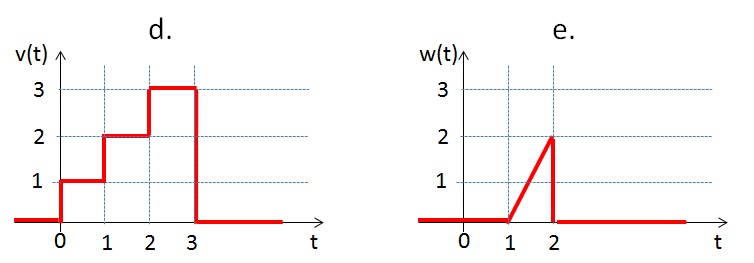
\includegraphics[scale=0.5]{images/Exo_2_1_a.jpg} 
	\end{figure} 
	
	\begin{figure}[h!]
		\centering
		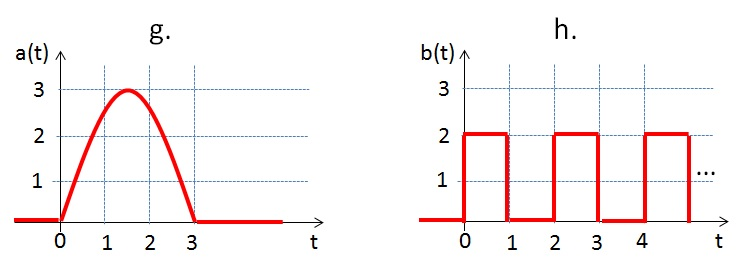
\includegraphics[scale=0.5]{images/Exo_2_1_b.jpg} 
	\end{figure}
	
	
	
	\vspace{1\baselineskip}
	
	\subsubsection{Exercice 2}
	
	Déterminez les expressions temporelles des fonctions suivantes :
	
	a. $X(p)=\frac{p-4}{p^{2}+16}$ 
	
	b. $Y(p) = \frac{p^{2}+3p+3-\frac{6}{p}}{p^{2}}$ 
	
	c. $Z(p) = \frac{p^{2}+4p+4}{p^{2}+2p+2}$
	
	d. $W(p) = \frac{p-1+e^{-p}}{p^{2}(1-e^{-p})}$. Tracez cette fonction.
	
	
	\vspace{1\baselineskip}
	
	\subsubsection{Exercice 3}
	
	Résoudre les équation différentielles suivantes :
	
	a. $x"+2x'+x=e^{-t}u(t)$, avec x(0) = 0 et x'(0) = 0. 
	
	b. $x"+6x'+8x=\delta(t)$ avec x(0)=1 et x'(0)=3. 
	
	\vspace{1\baselineskip}
	
	
	\subsubsection{Exercice 4}
	
	On reprend l'exercice 8 du chapitre 2.

	
	\begin{figure}[h!]
		\centering
		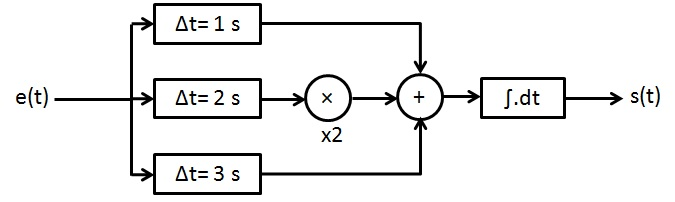
\includegraphics[scale=0.5]{images/Exo_2_6.jpg} 
	\end{figure}
	
	a. Ecrivez la fonction de transfert du système dans le domaine de Laplace.
	
	b. Calculez la réponse indicielle du système. On supposera que les conditions initiales de tous les nœuds internes du système sont nulles. 
	
	
	\vspace{1\baselineskip}
	
	\subsubsection{Exercice 5}
	
	On considère un circuit électrique, dont le courant i(t) est donné par l'équation ci-dessous.
	\begin{equation*}
	e(t)=\frac{d^{2}i}{dt^{2}}+7\frac{di}{dt}+10i(t)
	\end{equation*}
	On considère l'excitation suivante $e(t)=6e^{-3t}u(t)$. Les conditions initiales du circuit sont : $i(0) = 3~A$ et $\frac{di}{dt}(0)=3~A/s$.
	
	
	a. Etablir l'expression du courant dans le domaine de Laplace.
	
	b. En déduire l'expression temporelle du courant i(t).
	
	c. Vérifiez, en utilisant les expressions du courant dans le domaine de Laplace, puis dans le domaine temporel, que la condition initiale du courant est respectée. Déterminez ensuite les conditions finales. 
	
	\vspace{1\baselineskip}
	
	\subsubsection{Exercice 6 - Réponse d'un moteur à courant continu à aimants permanents}
	
	Le fonctionnement d'un moteur est gouverné par un modèle électromécanique, se présentant sous la forme de plusieurs équations différentielles reliant grandeurs électriques et mécaniques. Dans cet exercice, nous allons étudier le modèle simplifié d'un moteur à courant continu à aimants permanents. La figure ci-dessous présente le modèle électrique équivalent de l'induit. Celui-ci est modélisé par un circuit RL et est excité par une tension de commande notée $U_{C}$. Lorsque le moteur tourne, une force contre électromotrice (fcem) E est induite, qui est proportionnelle à la vitesse angulaire du moteur $\Omega$. 
	\begin{figure}[h!]
		\centering
		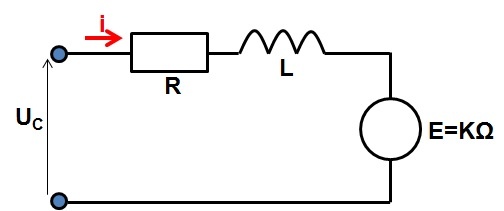
\includegraphics[scale=0.5]{images/Exo3_moteur.jpg} 
	\end{figure}	
	Le courant i circulant dans l'induit produit un couple moteur $C_{m}$, selon la même constante de proportionnalité K que celle liant la fcem et la vitesse de rotation du moteur. A ce couple moteur s'opposent plusieurs sources de couples résistants $C_{R}$ :
	\begin{itemize}
		\item l'inertie du moteur, donnée par le moment d'inertie J
		\item les frottements visqueux, caractérisés par le coefficient de frottement visqueux f
	\end{itemize}
	L'équation mécanique du moteur s'écrit alors :
	\begin{equation*}
	C_{m} = C_{R} = J\frac{d\Omega}{dt}+f\Omega
	\end{equation*}	
	Nous cherchons à déterminer la vitesse de rotation du moteur en fonction de l'excitation appliquée.
	Dans cet exercice, on considèrera les valeurs suivantes : r=0.2 $\Omega$, L = 0.2 mH, K = 0.057 N.m/A, J = $650.10^{-7}~kg.m^{2}$, f = $2.3.10^{-5}~N.m/rad.s^{-1}$. On suppose que le moteur est initialement à l'arrêt.\\
	
	a. Etablir l'équation différentielle reliant la vitesse de rotation et l'excitation $U_{C}$ du moteur.
	
	b. Déterminez la fonction de transfert du moteur dans le domaine de Laplace. Exprimez-la sous la forme $\frac{G}{p^{2}+2\alpha p+\omega_{0}^{2}}$.
	
	c. Calculez les pôles du système. Est-il stable ?
	
	d. En t = 0, on applique une commande de type échelon unitaire d'amplitude $Uc_{0}$ = 10 V. Déterminez l'expression du profil temporel de la vitesse angulaire.
	
	e. Esquissez le profil temporel de la vitesse angulaire. En régime permanent, quelle est la valeur de la vitesse ? 
	
		
	\newpage
	